The electronic noise of the sensor is estimated in runs acquired
with the sensor in complete dark ({\it pedestal} runs). For each
pixel, the pedestal is computed as the average of the counts over many
events \textcolor{red}{non sarebbe meglio chiamarli frames ? o images ? }, while the electronic noise is computed as the standard deviation
(SD) of the counts. The distribution of the pixels SD is shown in
Fig.~\ref{fig:noise}. The mode of this distribution is about 1.8
photons per pixels, but a tail is present, with pixels having a
 noise of more than 5 photons per pixels.
The pedestal $\mu_i$ is then subtracted to the image for each $i^th$ pixel.
An initial noise suppression is applied by neglecting the pixels with counts less than $1.3\times\textrm{SD}_i$.
%where $i$ represents the
%pixel (\textit{zero suppression}). 
%
\begin{figure}[ht]
  \centering
  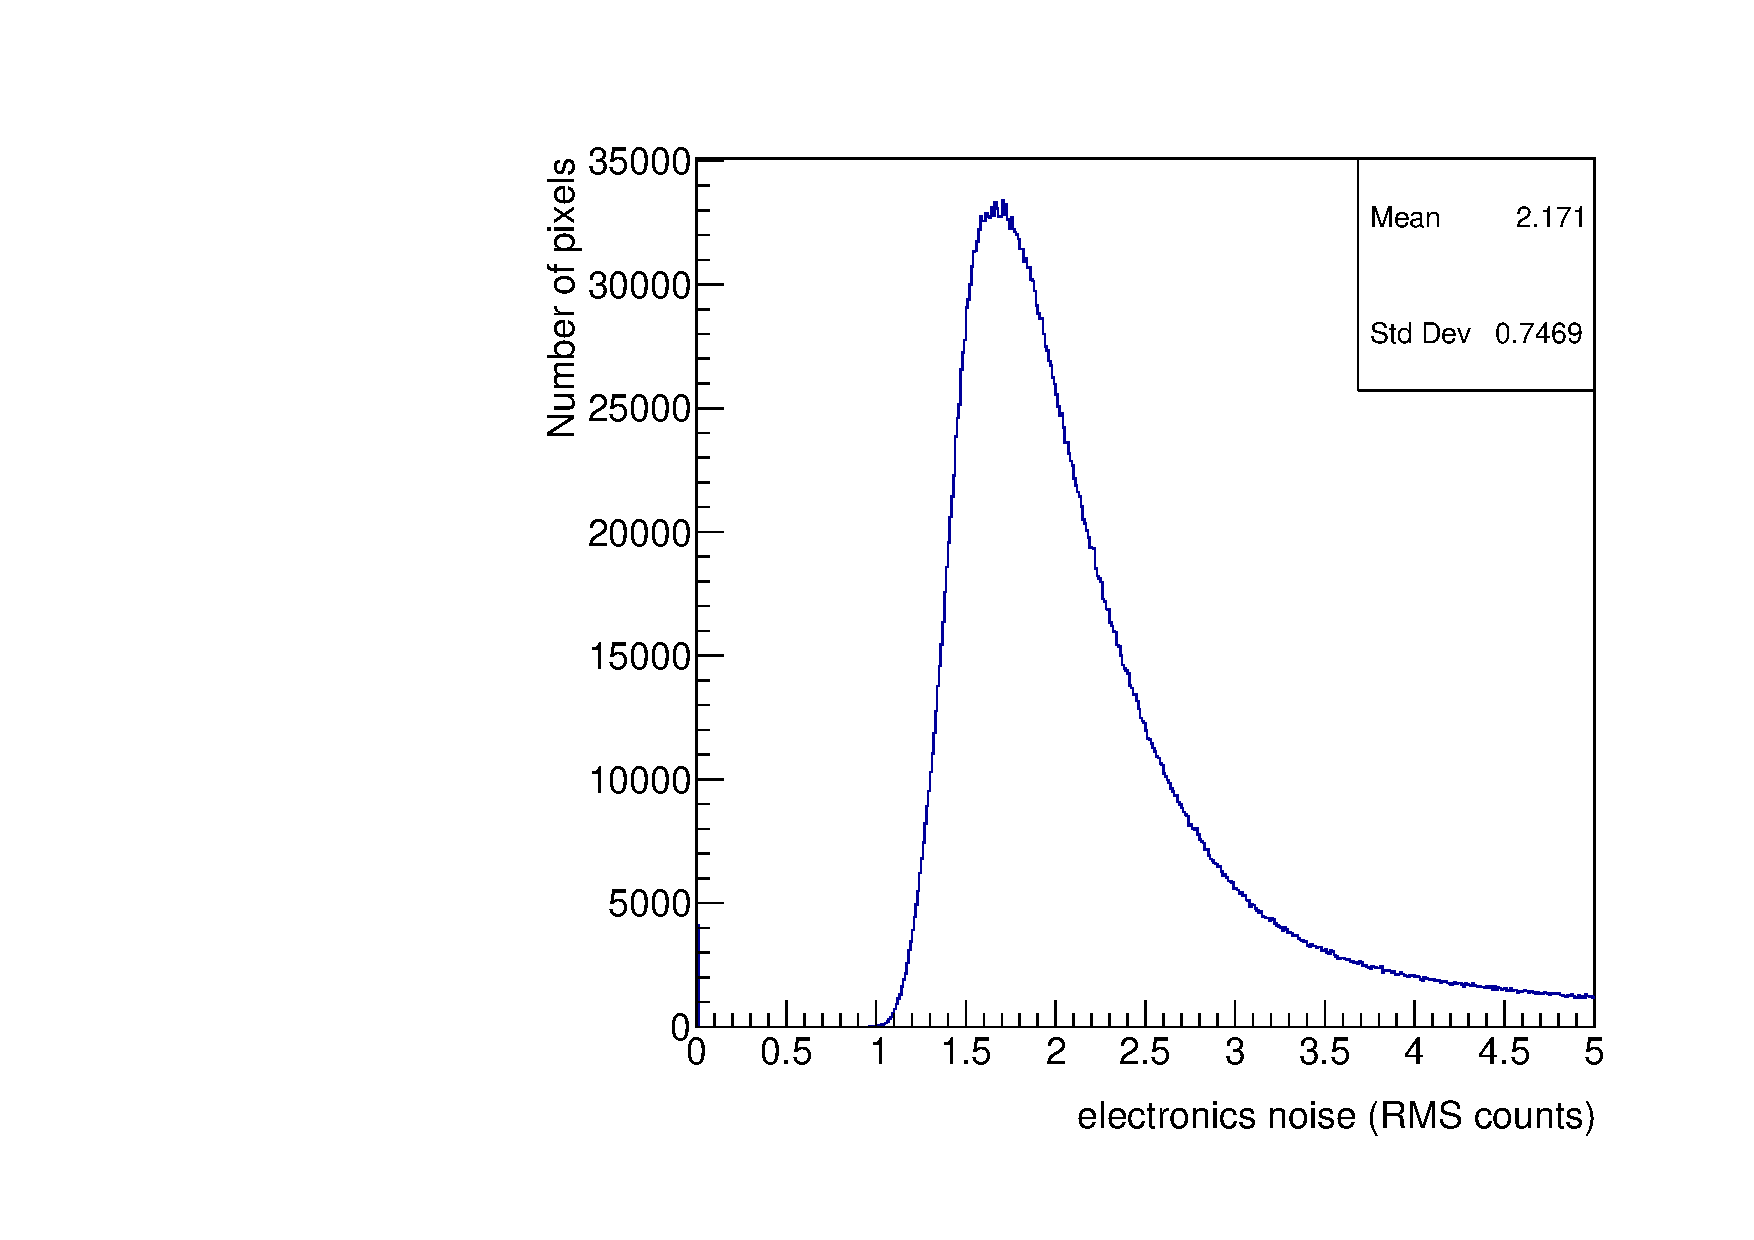
\includegraphics[width=0.45\linewidth]{figures/sensor_noise}
  \caption{Distribution of the electronic noise of the sensor,
    estimated in images taken with sensor in complete dark, and
    evaluated as the RMS of the distribution of the counts for each
    pixel.  \label{fig:noise}}
\end{figure}
%
On such pedestal-subtracted zero-suppressed images  an upper
threshold is applied to reject hot pixels, which are more likely due
to sensor instabilities than to energy deposition. These are not
malfunctional pixels  because they disappear after a
power cycle of the camera and therfore a dynamic (run-by-run) suppression is
needed.  The hot pixels are efficiently identified as high-intensity, isolated
pixels, and distinguished by a true energy deposit, for which each
pixel is surrounded by some other active pixels. A minimum average of
the counts, and a minimum number of two pixels above noise in a
$3\times3$ pixels matrix surrounding the hot pixel is required.
\textcolor{red}{is required to do what ? to retain the pixel ?}

The resolution of the resulting image is then reduced by creating
\textit{macro-pixels}, by averaging the counts in $4\times4$ pixel
matrices. This is needed to reduce the combinatorics   of the following
clustering algorithm to be executed   in a reasonable time for each
image. On such $512\times512$ pixel map, a median
filtering~\cite{medianfilter} is applied, as described in more details
in Ref.~\cite{medianfilter_cygno}. The output image is passed to the
basic clustering algorithm, described in the following.


